%% This LaTeX-file was created by <valette> Mon Feb 15 17:47:54 1999
%% LyX 1.0 (C) 1995-1999 by Matthias Ettrich and the LyX Team

%% Do not edit this file unless you know what you are doing.
\documentclass[10pt,american]{article}
\usepackage[T1]{fontenc}
\usepackage{a4wide}
\pagestyle{plain}
\usepackage{babel}
\usepackage[dvips]{graphics}

\makeatletter


%%%%%%%%%%%%%%%%%%%%%%%%%%%%%% LyX specific LaTeX commands.
\newcommand{\LyX}{L\kern-.1667em\lower.25em\hbox{Y}\kern-.125emX\@}

%%%%%%%%%%%%%%%%%%%%%%%%%%%%%% Textclass specific LaTeX commands.
\newenvironment{lyxcode}
  {\begin{list}{}{
    \setlength{\rightmargin}{\leftmargin}
    \raggedright
    \setlength{\itemsep}{0pt}
    \setlength{\parsep}{0pt}
    \ttfamily}%
   \item[]}
  {\end{list}}

%%%%%%%%%%%%%%%%%%%%%%%%%%%%%% User specified LaTeX commands.
\usepackage[dvips]{epsfig}

\makeatother

\begin{document}

\vspace{0.3cm}
{\par\centering \resizebox*{1\textwidth}{!}{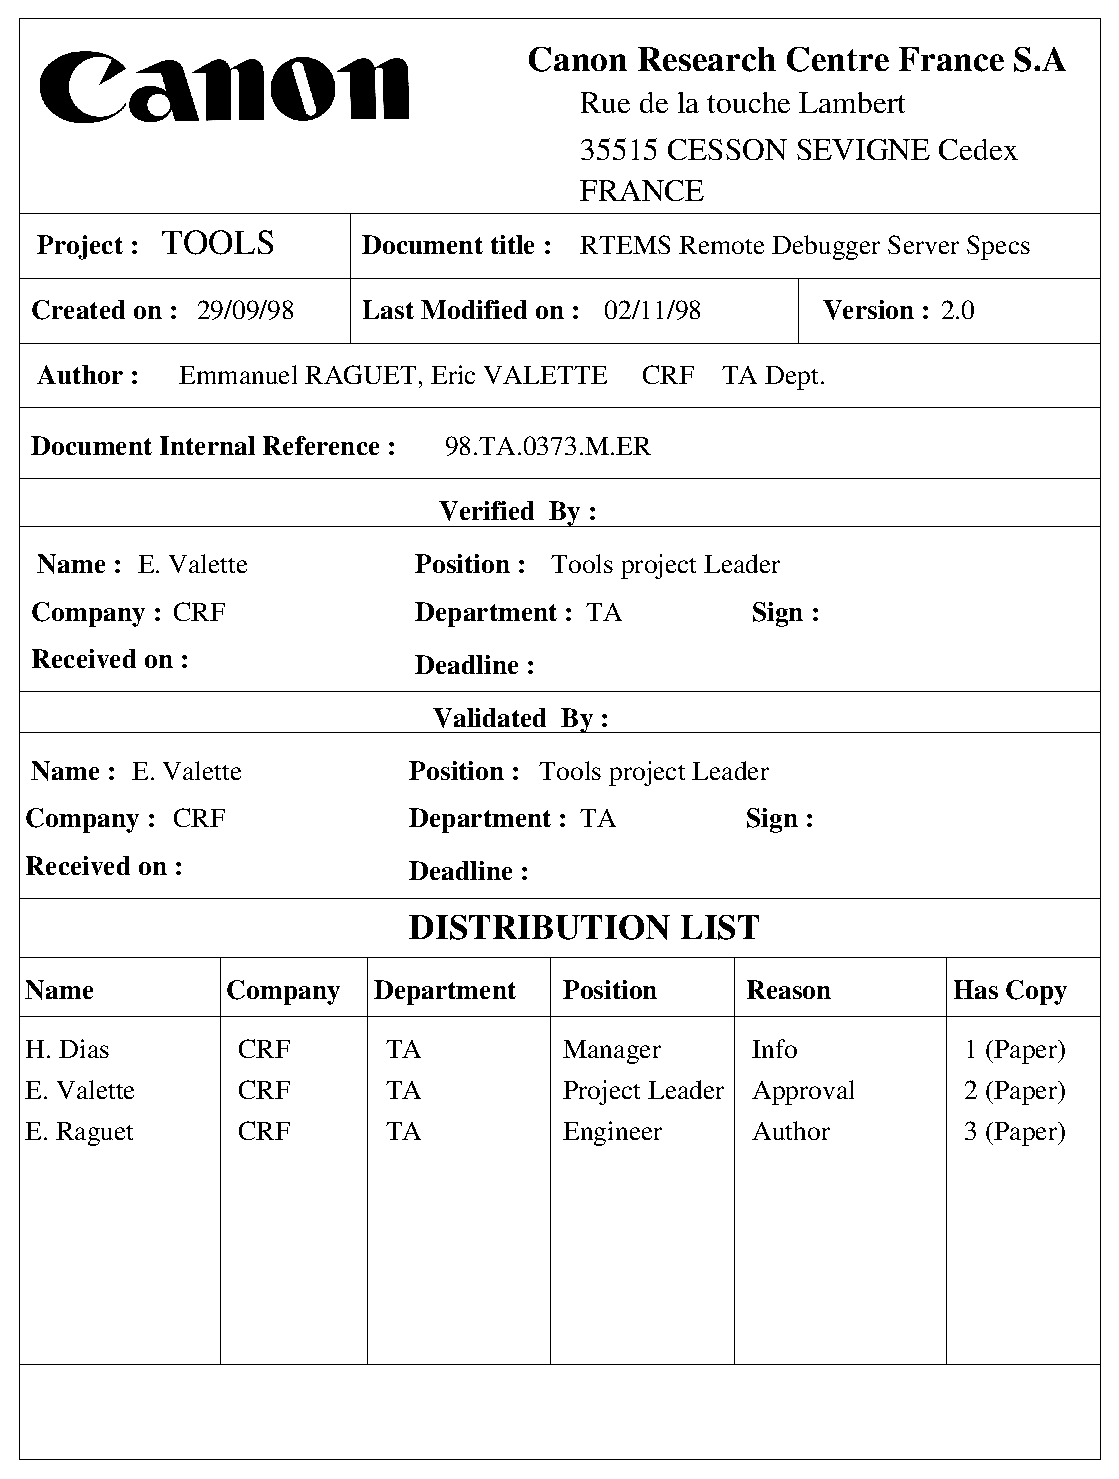
\includegraphics{garde.eps}} \par}

{\par\centering \newpage\par}
\vspace{0.3cm}

\bigskip{}
{\par\centering \textbf{\Huge RTEMS Remote Debugger}\Huge \par}
\bigskip{}

\tableofcontents

\listoffigures \newpage


\section{\noindent Introduction}

\noindent The TOOLS project aims to provide a complete development environment
for RTEMS OS. This environment must be as close as possible to the Chorus one
(gnu compiler, gnu linker, gnu debugger,~...), because it is currently the OS
which is the most used at CRF and we want to simplify the migration path from
the ChorusOs environment to the RTEMS environment. One important item of this
development environment is the remote debugger which allows the developer to
debug his software on a target machine from a host machine via a communication
link (Ethernet, serial link,~...). \\


\noindent The choice of GDB as debugger has been made with because in CRF, every
developer, which uses the ChorusOs development environment, debugs his software
using the remote debugging functionality of GDB. Providing a remote GDB debug
server running on RTEMS, will enable the developers to use transparently the
same debugger for a different RTOS. Another reason for the choice of GDB is
its constant evolution, and that it can be interfaced with graphic user interfaces
like DDD providing a very powerfull debugging environment.\\


\noindent The subject of this document is to explain how GDB works and the way
to implement a daemon on RTEMS that will be used as a debugger server for a
GDB client. We will call this daemon Rtems GDB Debug Server Daemon (RGDBSD).
We aim to provide this debugger running at least on 2 host systems : Linux 2.x
and Solaris 2.5.1 as they are the two platforms used for developing Chorus applications
today.


\section{\noindent Document Revision History}

\noindent \underbar{Current release} : 

\begin{itemize}
\item \noindent Current applicable release is 2.0.
\end{itemize}
\noindent \underbar{Existing releases} :

\begin{itemize}
\item \noindent 0.1 : Released the 29/09/98. First draft of this document.
\item \noindent 0.2 : Released the 05/10/98. Second draft version.
\item 1.0 : Released the 08/10/98. Version Approved internally.
\item 1.1 : Released the 13/13/98. Version Distributed for comments.
\item 2.0 : Released the 01/11/98. Version including modifications related to comments
we have got from the RTEMS mailing list. It also contains a more precise description
of RGDBSD as we now have a first prototype,
\end{itemize}
\noindent \underbar{Planned releases} :

\begin{itemize}
\item \noindent 2.1 Final specification release intended to include a second round
of comments,
\end{itemize}

\section{\noindent Objectives}

This section is intended to clearly define the current objectives of our work.
First, we will try here to list some ambitious requirements for the debugger
in section \ref{req_ref}. These requirements will deliberately be much more
ambitious than what we will provide directly ourselves in the hope that the
Internet development model will enable others to implement some features we
rejected for man-power reasons in the first step. We are committed to do the
core work and redistribute it but would appreciate any comment and enhancement.
Then, in section \ref{req_anal_ref} we will analyze each requirement to see
what technical problem must be solved if we want to fullfill it. After this
analysis, we will determine in section \ref{Sel_req_ref} the requirements we
chose to implement and the ones we will not. We will then clearly identify the
limits of our solution in section \ref{REstric_ref}.


\subsection{\noindent \label{req_ref}List of Requirements}

We will identify here possible requirements for the type of debug that may be
provided :

\begin{description}
\item [(R1)]: We want to use GDB as the front-end debugger,
\item [(R2)]: We want to support at least Intel and PowerPC as target processor architecture,
\item [(R3)]: We want to use the GDB thread debugging interface,
\item [(R4)]: We want to be able to debug a remote target over a serial line,
\item [(R5)]: We want to be able to debug a remote target over Ethernet,
\item [(R6)]: The set of target code path we will be able to debug using RGDBSD must
be clearly identified. It will be called Debug Path Set (\emph{DPS}) in the
remaining of this document,
\item [(R7)]: \emph{DPS} must include the RTEMS core executive itself,
\item [(R8)]: \emph{DPS} must include the FreeBSD stack, 
\item [(R9)]: \emph{DPS} must include anything but the FreeBSD stack and the RTEMS
core executive,
\item [(R10)]: We want to enable several persons to debug different parts of the code
running on the target,
\item [(R11)]: As much as possible the system must be frozen during a debug session
so that debugging a particular portion of code does not prevent another part
from functioning,
\end{description}

\subsection{\noindent \label{req_anal_ref}Requirements Analysis}

\begin{description}
\item [(R1)]: Worth recalling it. It mainly imposes few restrictions on the binary
files type, target processor type as :

\begin{itemize}
\item the binary format must be understood by GDB (to find debugging information).
Elf, Coff and A.out are the main formats currently supported. Elf/Dwarf 2.0
binary support will be our main target as they are the preferred format for
Intel and PowerPC processors. No change in GDB will be required for other binaries
except may be a new configuration file changing the binary/debug file format,
\item the processor must be supported for disassemble/step instruction command,
\item the target system must be supported. As far as I know RTEMS is not currently
\emph{officially} supported anyway,
\end{itemize}
\item [(R2)]: Our primary targets are Intel and PowerPC. We however do not think implementing
RGDBSD for other processors will be a heavy task. It will mainly require :

\begin{enumerate}
\item Implementing exception handling for the target processor, 
\item Interfacing the generic part of RGDBSD with the low level exception handling
and make RGDBSD aware of exception used for debugging (usually illegal instruction
or dedicated trap, single step),
\item Making GDB aware of the frame layout pushed on exceptions,
\item Implement the code for data transfer for the exception frame,
\item Implement code to copy data cache back to main memory and invalidate instruction
cache. This is needed in order to be sure opcode modification used to set breakpoint
that use the data cache will be proagated to the instruction cache,
\end{enumerate}
As soon as we will have completed the first core work a document describing
how to port it to a new processor should be written. So far we will organize
the source tree with processor dependent directories so that port will be as
easy as possible. May be a bare processor support should be created,

\item [(R3)]: GDB already has an interface for manipulating multi-threaded programs.
This interface is rather weak at the moment but it will certainly be improved
in the future with the generalization of POSIX thread API on Linux and other
operating systems. This implies that either GDB or RGDBSD is able to obtain
the list of threads currently executing. The choice of implementing this in
GDB or RGDBSD is a tradeof between target code size and simplicity,
\item [(R4)]: Regular GDB code contains clients code for debugging over a serial line.
However only few functions are implemented. We would like to provide a better
support and to uniformize serial line debugging with debugging over Ethernet
via the use of SLIP,
\item [(R5)]: Regular GDB code contains client code for debugging over Ethernet for
VxWorks via the SUN RPC library. So there will be at least one starting point
to implement remote debugging over Ethernet via SUN RPC. The Chorus remote debugging
code has been disclosed under GPL and also contains code for debugging suing
SUN RPC,
\item [(R6)]: Due to a classical chicken and egg problems, the remote debugging daemon
cannot be used to debug code it uses to function. Thus depending on the API
used by RGDBSD, some parts of the target system will not be debuggable via GDB.
The most important point is documentation because my feeling is that implementing
RGDBSD on a totally different \emph{dedicated} nano kernel should be possible,
\item [(R7)]: RTEMS core executive is a real-time OS which implements priority level
scheduling, synchronization objects, and interrupt handling. As mentioned in
previous item, we may not debug theses features if RGDBSD uses them. This requirement
is thus very strong because it impose that :

\begin{enumerate}
\item RGDBSD is totally interrupt driven (no thread API available),
\item But it does not use RTEMS interrupt management,
\item Nor does not use RTEMS exception management,
\item RGDBSD must provide its own UDP/IP stack as the current FreeBSD code rely on
tasks switching and RTEMS provided synchronization object for input path handling,
\end{enumerate}
So our feeling is that the \textbf{(R7)} more or less requires to write a \emph{dedicated}
nano kernel with a very small dedicated UDP/IP stack.

\item [(R8)]: GDB remote debugging over Ethernet code communicates with the remote
target via the SUN RPC protocol. This requires a UDP/IP protocol and a minimal
socket like interface. In RTEMS environment, this feature is currently provided
by the FreeBSD stack. Again, if we use the FreeBSD stack itself for remote communication,
it will be impossible to debug this stack as a breakpoint in the stack code
will stop its execution and there would be no more way to communicate with the
target. A solution consists in implementing a minimal, dedicated UDP/IP stack
(with at least IP and UDP protocols, a minimal BSD sockets) and a simple SUN
RPC library, which will be both dedicated to the debug. We can use RTEMS API
to implement it if \textbf{(R7)} is not required. As the two stack will need
to share the same chip, a kind of shared filter must be implemented at the bottom
of the two stacks so that Ethernet frames can be dynamically directed either
to the dedicated UDP/IP debug stack or to the regular FreeBSD stack. The fact
that in the current design, the low level ethernet input routine mainly signal
a thread should facilitate the design of this filter. The output path is less
complicated as it is run by a task and thus can sleep on a synchronization object,
\item [(R9)]: This requirement represents what we find reasonable as a first target.
However, we can still present to the final user this kind of debugging via different
model. RTEMS can be represented as a single threaded system or, because RTEMS
is a multitasking system, as an ensemble of separate tasks. In the first representation,
the debugger sees only 1 ``task'' without distinguishing the core executive
part from the applicative part. This is the simplest way to implement the debugger
but also implies that there is no way to protect the core executive. Some of
these tasks are system tasks (tasks form the core executive and from the FreeBSD
stack), the other ones are tasks implemented by the developer. The developer
wants to debug his tasks, and sometimes only one of his tasks. We can provide
a way to debug not the entire system but only the concerned task by testing
if the current running task is a debugged task (test on the task identifier).
GDB offers an API to ``detach'' thread so that if a detached thread hits a
breakpoint it is automatically restarted without user intervention,
\item [(R10)]: Several developers can work on a large project, each on a specific
module. Sometimes only one target is available for everyone. This requirements
is not really meaningfull until RTEMS supports dynamic code loading,
\item [(R11)]: This requirement heavily depends on the \textbf{(R7)} and \textbf{(R8)}
requirements.
\end{description}

\subsection{\label{Sel_req_ref}Requirements Selection}


\subsubsection{Requirement We Will Take Into Account For the First Implementation}

\begin{description}
\item [(R1)]: Obviously.
\item [(R2)]: As these are our targets. Of course other will be free to contribute.
We will however document the works that needs to be done in order to port the
debug code to other processors,
\item [(R3)]: We think it is feasible with only few RTEMS modifications,
\item [(R5)]: We think serial line debugging is nowadays too restrictive as most equipment
are now connected via Ethernet,
\item [(R6)]: This is a documentation problem and should be fairly easy to describe
once we have the RGDBSD code,
\item [(R9)]: We will try to provide the multi-thread target system presentation,
\end{description}

\subsubsection{Requirements We Will Not Implement}

\begin{description}
\item [(R4)]: it will not be implemented for the moment. It is just a matter on implementing
SLIP in the FreeBSD stack and alternative solutions already exist in the meantime,
\item [(R7)]: To simplify the first developments, we don't plan to implement a \emph{dedicated}
nano-kernel to allow the RTEMS kernel to be debugged. It means that, if any
breakpoint is set in the kernel, unpredictable behaviors can occur. So, developers
must keep in mind to avoid stopping the kernel. They must also keep in mind,
in order to not stop the kernel, that the user's tasks must have a lower priority
than the tasks used for debug. The solution is to use a specific very-high priority
level for the system tasks used directly or indirectly by RGDBSD. The SYSTEM\_TASK
attribute that already exists should be fine.
\item [(R8)]: To avoid increasing the code size and the used memory and because the
FreeBSD stack doesn't need to be debug any more, we choose not to implement
a minimal TCP/IP stack but rather to use the FreeBSD one as communication protocol,
\item [(R10)]: We will see later when a file system will be available and we can implement
\textbf{exec} system call,
\item [(R11)]: Without a separate TCP/IP stack it will be hard to freeze the system
as some interrupts must occur in order to enable the FreeBSD stack to function,
\end{description}

\subsection{\noindent \label{REstric_ref}Implied Restrictions}

\noindent High priority level must be used for these features :

\begin{itemize}
\item \noindent FreeBSD interrupt handling thread,
\item \noindent Debugger threads.
\end{itemize}
\noindent This will allows these tasks not to be stopped when a process is stopped
in debug mode 

\noindent If we don't want to use a ``specific'' priority level, we must affect
priority to each of these tasks as follow :

\begin{itemize}
\item \noindent FreeBSD stack (high priority)
\item \noindent Debugger (less high priority)
\end{itemize}
\noindent The user must remember the higher priority level he can use for his
software in order not to block one of the previous threads and to not put breakpoints
in part of the code executed by RGDBSD.


\section{\noindent A Rapid Tour of GDB Internals}

\noindent To help the reader to understand what needs to be implemented, we
will present briefly how GDB works regardless if the target is local or remote.
A debugger is a tool which enables control of the execution of software on a
target system. In most of cases, the debugger connects to a target system, attaches
a process, inserts breakpoints and resumes execution. Then the normal execution
is completely events driven (process execution stopped due to a breakpoint,
process fault, single-step,...) coming from the debuggee. It can also directly
access some parts of the target processor context (registers, data memory, code
memory,...) and change their content. Native GDB debugger can just be seen as
special cases where the host and the target are on the same machine and GDB
can directly access the target system debug API.\\


\noindent In our case, the host and the target are not on the same machine and
an Ethernet link is used to communicate between the different machines. Because
GDB needs to be able to support various targets (including Unix core file, ...),
each action that needs to be performed on the debuggee is materialized by a
field of the following \emph{targets\_op}s structure : 

\begin{lyxcode}
{\par\noindent struct~target\_ops\par}

{\par\noindent \{\par}

{\par\noindent ~~char~~~~~~~~~{*}to\_shortname;~~~/{*}~Name~this~target~type~{*}/\par}

{\par\noindent ~~char~~~~~~~~~{*}to\_longname;~~~~/{*}~Name~for~printing~{*}/\par}

{\par\noindent ~~char~~~~~~~~~{*}to\_doc;~~~~~~~~~/{*}~Documentation.~~Does~not~include~trailing\par}

{\par\noindent ~~~~~~~~~~~~~~~~~~~~~~~~~~~~~~~~~~~newline,~and~starts~with~a~one-line~descrip-\par}

{\par\noindent ~~~~~~~~~~~~~~~~~~~~~~~~~~~~~~~~~~~tion~(probably~similar~to~to\_longname).~{*}/\par}

{\par\noindent ~~void~~~~~~~~({*}to\_open)~PARAMS~((char~{*},~int));\par}

{\par\noindent ~~void~~~~~~~~({*}to\_close)~PARAMS~((int));\par}

{\par\noindent ~~void~~~~~~~~({*}to\_attach)~PARAMS~((char~{*},~int));\par}

{\par\noindent ~~void~~~~~~~~({*}to\_detach)~PARAMS~((char~{*},~int));\par}

{\par\noindent ~~void~~~~~~~~({*}to\_resume)~PARAMS~((int,~int,~enum~target\_signal));\par}

{\par\noindent ~~int~~~~~~~~~({*}to\_wait)~PARAMS~((int,~struct~target\_waitstatus~{*}));\par}

{\par\noindent ~~void~~~~~~~~({*}to\_fetch\_registers)~PARAMS~((int));\par}

{\par\noindent ~~void~~~~~~~~({*}to\_store\_registers)~PARAMS~((int));\par}

{\par\noindent ~~void~~~~~~~~({*}to\_prepare\_to\_store)~PARAMS~((void));\par}

{\par\noindent ~\par}

{\par\noindent ~~/{*}~Transfer~LEN~bytes~of~memory~between~GDB~address~MYADDR~and\par}

{\par\noindent ~~~~~target~address~MEMADDR.~~If~WRITE,~transfer~them~to~the~target,~else\par}

{\par\noindent ~~~~~transfer~them~from~the~target.~~TARGET~is~the~target~from~which~we\par}

{\par\noindent ~~~~~get~this~function.\par}

{\par\noindent ~\par}

{\par\noindent ~~~~~Return~value,~N,~is~one~of~the~following:\par}

{\par\noindent ~\par}

{\par\noindent ~~~~~0~means~that~we~can't~handle~this.~~If~errno~has~been~set,~it~is~the\par}

{\par\noindent ~~~~~error~which~prevented~us~from~doing~it~(FIXME:~What~about~bfd\_error?).\par}

{\par\noindent ~\par}

{\par\noindent ~~~~~positive~(call~it~N)~means~that~we~have~transferred~N~bytes\par}

{\par\noindent ~~~~~starting~at~MEMADDR.~~We~might~be~able~to~handle~more~bytes\par}

{\par\noindent ~~~~~beyond~this~length,~but~no~promises.\par}

{\par\noindent ~\par}

{\par\noindent ~~~~~negative~(call~its~absolute~value~N)~means~that~we~cannot\par}

{\par\noindent ~~~~~transfer~right~at~MEMADDR,~but~we~could~transfer~at~least\par}

{\par\noindent ~~~~~something~at~MEMADDR~+~N.~~{*}/\par}

{\par\noindent ~\par}

{\par\noindent ~~int~~~~~~~~~({*}to\_xfer\_memory)~PARAMS~((CORE\_ADDR~memaddr,~char~{*}myaddr,\par}

{\par\noindent ~~~~~~~~~~~~~~~~~~~~~~~~~~~~~~~~~~~~~~~~~int~len,~int~write,\par}

{\par\noindent ~~~~~~~~~~~~~~~~~~~~~~~~~~~~~~~~~~~~~~~~~struct~target\_ops~{*}~target));\par}

{\par\noindent ~\par}

{\par\noindent ~~void~~~~~~~~({*}to\_files\_info)~PARAMS~((struct~target\_ops~{*}));\par}

{\par\noindent ~~int~~~~~~~~~({*}to\_insert\_breakpoint)~PARAMS~((CORE\_ADDR,~char~{*}));\par}

{\par\noindent ~~int~~~~~~~~~({*}to\_remove\_breakpoint)~PARAMS~((CORE\_ADDR,~char~{*}));\par}

{\par\noindent ~~void~~~~~~~~({*}to\_terminal\_init)~PARAMS~((void));\par}

{\par\noindent ~~void~~~~~~~~({*}to\_terminal\_inferior)~PARAMS~((void));\par}

{\par\noindent ~~void~~~~~~~~({*}to\_terminal\_ours\_for\_output)~PARAMS~((void));\par}

{\par\noindent ~~void~~~~~~~~({*}to\_terminal\_ours)~PARAMS~((void));\par}

{\par\noindent ~~void~~~~~~~~({*}to\_terminal\_info)~PARAMS~((char~{*},~int));\par}

{\par\noindent ~~void~~~~~~~~({*}to\_kill)~PARAMS~((void));\par}

{\par\noindent ~~void~~~~~~~~({*}to\_load)~PARAMS~((char~{*},~int));\par}

{\par\noindent ~~int~~~~~~~~~({*}to\_lookup\_symbol)~PARAMS~((char~{*},~CORE\_ADDR~{*}));\par}

{\par\noindent ~~void~~~~~~~~({*}to\_create\_inferior)~PARAMS~((char~{*},~char~{*},~char~{*}{*}));\par}

{\par\noindent ~~void~~~~~~~~({*}to\_mourn\_inferior)~PARAMS~((void));\par}

{\par\noindent ~~int~~~~~~~~~({*}to\_can\_run)~PARAMS~((void));\par}

{\par\noindent ~~void~~~~~~~~({*}to\_notice\_signals)~PARAMS~((int~pid));\par}

{\par\noindent ~~int~~~~~~~~~({*}to\_thread\_alive)~PARAMS~((int~pid));\par}

{\par\noindent ~~void~~~~~~~~({*}to\_stop)~PARAMS~((void));\par}

{\par\noindent ~~enum~strata~~~to\_stratum;\par}

{\par\noindent ~~struct~target\_ops\par}

{\par\noindent ~~~~~~~~~~~~~~~~{*}DONT\_USE;~~~~~~/{*}~formerly~to\_next~{*}/\par}

{\par\noindent ~~int~~~~~~~~~~~to\_has\_all\_memory;\par}

{\par\noindent ~~int~~~~~~~~~~~to\_has\_memory;\par}

{\par\noindent ~~int~~~~~~~~~~~to\_has\_stack;\par}

{\par\noindent ~~int~~~~~~~~~~~to\_has\_registers;\par}

{\par\noindent ~~int~~~~~~~~~~~to\_has\_execution;\par}

{\par\noindent ~~struct~section\_table\par}

{\par\noindent ~~~~~~~~~~~~~~~{*}to\_sections;\par}

{\par\noindent ~~struct~section\_table\par}

{\par\noindent ~~~~~~~~~~~~~~~{*}to\_sections\_end;\par}

{\par\noindent ~~int~~~~~~~~~~~to\_magic;\par}

{\par\noindent ~~/{*}~Need~sub-structure~for~target~machine~related~rather~than~comm~related?~{*}/\par}

{\par\noindent \};\par}
\end{lyxcode}
\noindent This structure contains pointers to functions (in C++, this would
be called a virtual class). Each different target supported by GDB has its own
structure with the relevant implementation of the functions (some functions
may be not implemented). When a user connects GDB to a target via the ``target''
command, GDB points to the structure corresponding to this target. Then the
user can attache GDB to a specific task via the ``attach'' command. We have
therefore identified two steps to begin a remote debug session :

\begin{enumerate}
\item the choice of the target type (in our case RTEMS),
\item the choice of what to debug (entire system, specific task,...),
\end{enumerate}
Note that in the case of natives debugger, the choice of the target is implicitly
performed by commands like \textbf{run}, \textbf{attach}, \textbf{detach}. Several
figures will now be described showing the main steps of a debug session. \newline

\noindent Figure \ref{init_seq} explains how the debugger connects to the target
:

\begin{enumerate}
\item \noindent The debugger opens a connection to the target. The word ``connection''
doesn't only mean Ethernet or serial link connection but all the ways by which
a process can communicate with another one (direct function call, messages mailbox,
...),
\item \noindent The targets checks if it can accept or reject this connection,
\item \noindent If the connection is accepted, the host ``attaches'' the process,
\item \noindent the target stops the process, notifies a child's stop to the host
and waits for command,
\item \noindent the host can ask information about the debugged process (name, registers,...)
or perform some action like setting breakpoints, ...
\end{enumerate}
\noindent Figure \ref{breakpoint seq} explains how the debugger manages the
breakpoints and controls the execution of a process :

\begin{enumerate}
\item \noindent The host asks the debuggee what is the opcode at the concerned address
in order for GDB to memorize this instruction,
\item \noindent the host sends a CONTINUE command : it asks the target to write the
``DEBUG'' opcode (for example, the INTEL ``DEBUG'' opcode is INT3 which
generate a breakpoint trap) instead of the debugged opcode.
\item \noindent then the host waits for events,
\item \noindent after the change of instruction, the target resumes the execution
of the debuggee,
\item \noindent when the ``DEBUG'' opcode is executed, the breakpoint exception
handler is executed and it notifies the host that the process is stopped. Then
it waits for commands (if no command is sent after a certain amount of time,
the connection will be closed by the target).
\item \noindent the host asks the target to re-write the right opcode instead of the
''DEBUG'' opcode and then can ask information
\end{enumerate}
\noindent Figure \ref{breakpoint seq} also shows the case of other ``CONTINUE''
commands (remember that the ``DEBUG'' opcode has been replaced by the right
instruction): 

\begin{enumerate}
\item \noindent Host sends first a ``single step'' command to execute the debugged
instruction,
\item \noindent It then waits for ``single step`` exception event,
\item \noindent the target, once the single step executed, calls the debug exception
handler. It notifies the host that execution is suspended and wait for commands.
\item \noindent the host asks the target to re-write the ``DEBUG'' opcode (breakpoint
trap) instead of the debugged one.
\item \noindent then the host sends a ``CONTINUE'' command in order the target to
resume the process execution to the next breakpoint.
\end{enumerate}
\noindent Figure \ref{detach seq} explains how the debugger disconnects from
a target :

\begin{enumerate}
\item \noindent the host sends a detach command to the target.
\item \noindent the target detaches the concerned process, notifies the detachment
and resumes the process execution.
\item \noindent once notified, the host sends a close connection command.
\item \noindent the target closes the connection.
\end{enumerate}
\noindent These 3 examples show that the mains actions that are performed by
the host debugger on the target are only simple actions which look like :

\begin{itemize}
\item \noindent read/write code,
\item \noindent read/write data,
\item \noindent read/write registers,
\item \noindent manage exceptions,
\item \noindent send/receive messages to/from the host. 
\begin{figure}
{\par\centering \resizebox*{1\textwidth}{0.7\textheight}{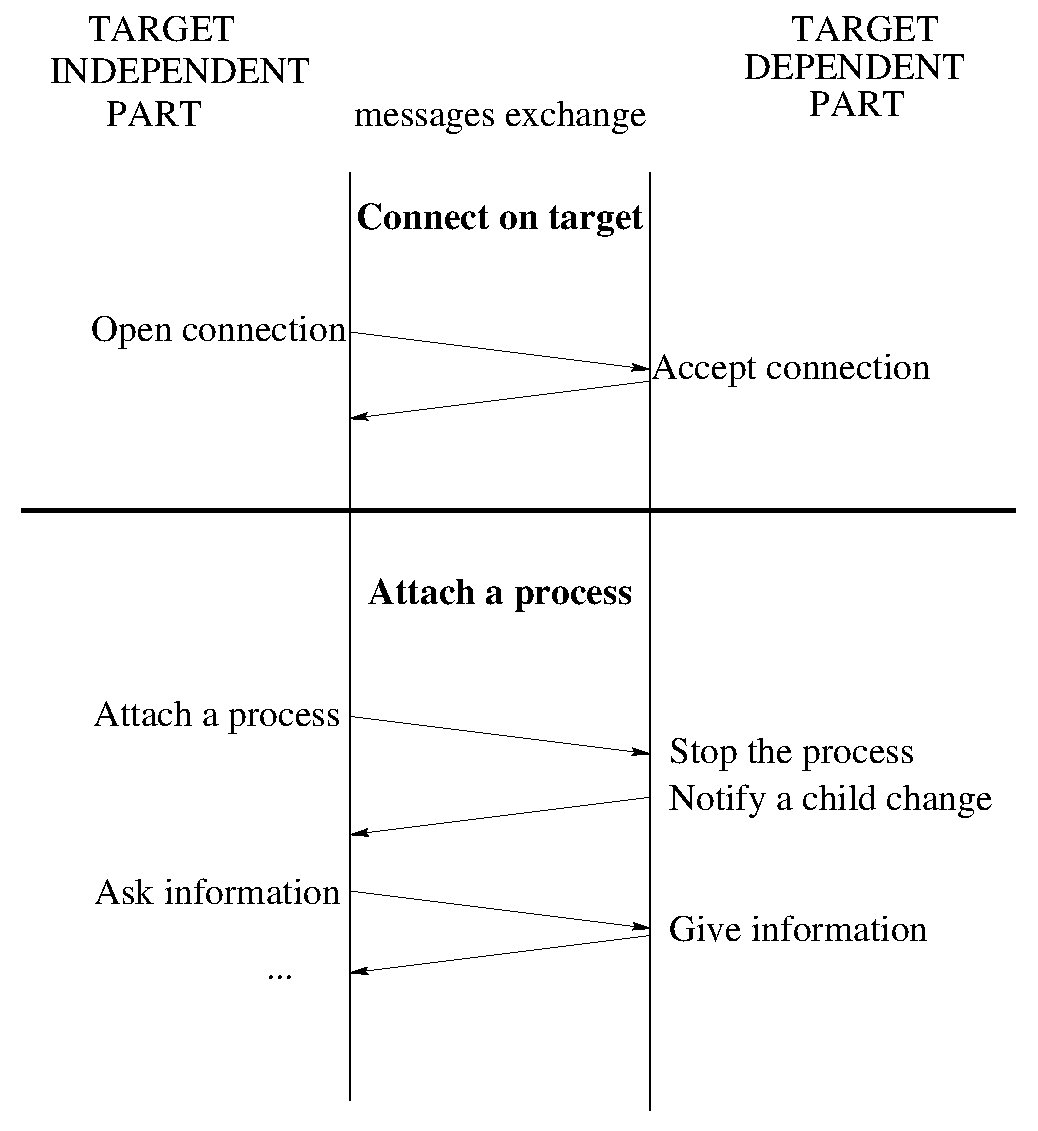
\includegraphics{seg_init.eps}} \par}


\caption{\label{init_seq}Debug session initialization}
\end{figure}
\begin{figure}
{\par\centering \resizebox*{0.8\textwidth}{1\textheight}{\includegraphics{seq_break.eps}} \par}


\caption{\label{breakpoint seq}Breakpoint and process execution}
\end{figure}
\begin{figure}
{\par\centering \resizebox*{0.7\textwidth}{0.3\textheight}{\includegraphics{seq_detach.eps}} \par}


\caption{\label{detach seq}Detach a process and close a connection}
\end{figure}

\end{itemize}

\section{\noindent Interfacing GDB with RTEMS as a Target}

\noindent So, basically, porting GDB to RTEMS environment requires implementing
the functions contained in the target\_ops structure. The native debugger implementation
(where the host machine is also the target one) uses direct function calls.
For our needs (remote debugging), these functions must be implemented to support
the encapsulation in UDP/IP layers and communications between different types
of host machines : the best solution is use the SUN Remote Procedure Calls API
(SUN RPC). This SUN RPC module will be explained below (see paragraph \ref{RPC}).

\noindent We can note that the functions described in the target\_ops structure
are high-level functions. The main reason is that GDB was designed in order
to be able to use monitor firmware as a debug server. In the case of a Unix
OS target, these high-level functions are implemented themselves using a lower
level POSIX API. Because we want to simplify the code running on the target
and decrease its size of this code, we propose to use the POSIX layer API used
for the debug like \textbf{waitpid}, \textbf{ptrace},~... Due to the GDB working
mode and due to our requirements, we can establish here a non-exhaustive list
of some commands required to implement the previously described functions~:

\begin{itemize}
\item \noindent set up a connection with a target,
\item \noindent close a connection,
\item \noindent send a signal to the specified process,
\item \noindent get a list of process/thread/connection running,
\item \noindent control process under debug,
\item \noindent ...
\end{itemize}
\noindent Control means that, with this function, we can read, write the memory
of the debuggee, insert breakpoint to stop the process and resume the process
execution. This command can be implemented by emulating in the RTEMS environment
a Unix function called ``ptrace''. This function allows the control of a child
process. The ``ptrace'' function has some sub-functions which are described
below (some of these actions and standardized, the others are added due to our
needs)~:

\begin{itemize}
\item \noindent PTRACE\_PEEKTEXT, PTRACE\_PEEKDATA : read word at address,
\item \noindent PTRACE\_POKETEXT, PTRACE\_POKEDATA :write word at address,
\item \noindent PTRACE\_CONT : restart after signal,
\item \noindent PTRACE\_KILL : send the child a SIGKILL to make it exit,
\item \noindent PTRACE\_SINGLESTEP : set the trap flag for single stepping,
\item \noindent PTRACE\_ATTACH : attach to the process specified,
\item \noindent PTRACE\_DETACH : detach a process that was previously attached.\newpage
\end{itemize}
\noindent This list only contains the command that are described in the ptrace
Unix manpage. For some specific needs (debug of one task among several ones,
register read/write,...), it is possible to create some special ptrace commands
as described after~:

\begin{itemize}
\item \noindent get current task registers,
\item \noindent set current task registers,
\item \noindent list of the threads,
\item \noindent identifier of the target thread,
\item \noindent restart to address,
\item \noindent set breakpoint at address,
\item \noindent clear breakpoint,
\item \noindent get breakpoints,
\item \noindent load dynamically a task,
\item \noindent ...
\end{itemize}
\noindent This list is not exhaustive and can be increased due to the needs.
All the described functions will not be implemented in a first version, only
the strictly needed. If some commands are added, the modifications must be implemented
both in RTEMS and in GDB.


\section{\noindent \label{RPC}Communication with GDB}

\noindent The RTEMS remote debugger will be accessed by GDB on a host machine
through a communication link. We will use the TCP/IP stack included in RTEMS
: the FreeBSD stack. The communication link will be based based on the UDP protocol
and the BSD sockets which are parts of the FreeBSD stack. On top of these layers,
we will plug a module which allows a simple communication between different
machines (especially between different endianess machines)~: the SUN Remote
Procedure Call (SUN RPC). This code is freely available on the net and comes
with a BSD like license. With this module, a process can invoke a procedure
on a remote system. The RTEMS remote debugger will be seen by GDB as a SUN RPC
server. Commands will be packed by the GDB SUN RPC client and sent to the server.
This server will unpack these commands, execute them and, if needed, return
results to the SUN RPC client.\\


\noindent Only a minimal subset of the SUN RPC library must be implemented.
For example, the portmapper related API which allows a dynamic allocation of
port numbers will not be implemented and some specific UDP port numbers will
be used to establish the communication between the host and the target. The
SUN RPC library implements the XDR module (eXternal Data Representation) which
is a standard way of encoding data in a portable fashion between different endian
systems. Below are figures describing the additional code and data size for
the minimal library implementation we currently have already implemented for
RTEMS :

\begin{lyxcode}
size~-x~librpc.a~

text~~data~bss~dec~hex~filename~

0x40e~0x0~0x0~1038~40e~rpc\_callmsg.o~(ex~librpc.a)~

0x2f1~0x18~0x0~777~309~rpc\_prot.o~(ex~librpc.a)~

0x458~0x0~0x0~1112~458~svc.o~(ex~librpc.a)~

0x4f~0x4~0x0~83~53~svc\_auth.o~(ex~librpc.a)~

0x75c~0x18~0x0~1908~774~svc\_udp.o~(ex~librpc.a)~

0x711~0x4~0x10~1829~725~xdr.o~(ex~librpc.a~

0x149~0x0~0x0~329~149~xdr\_array.o~(ex~librpc.a)~

0x165~0x20~0x0~389~185~xdr\_mem.o~(ex~librpc.a)
\end{lyxcode}
\noindent We have a constraint with the use of the UDP protocol. Because this
protocol is connectionless, it is impossible, especially for the target, to
detect if the connection is always active. On the other hand, using the TCP/IP
protocols seems to be heavy especially if we plan to implement a dedicated micro
stack for debug in the future. It can be a real problem to let the debugged
process stopped during a long time even if there is no more debugger connected
to the system. To avoid such a problem, the target must periodically test the
connection with the host on another way than the one used to receive the commands.
We must therefore open two communication ways so we need two fixed UDP port
numbers. 

\begin{enumerate}
\item \noindent One port will be used by the debugger to send its commands to the
debugged process and to receive the result of these commands. View from the
remote debugger, this port will be called primary port. For this one, we choose
arbitrarily the port number 2000. 
\item \noindent The other socket will be used as secondary port by the target to sometimes
test the connection between the host and the target. These tests will occur
in specific situations, when a process will be stopped on a breakpoint, single
step instruction or other means. This secondary port will also be used by the
target to signal any change in the behavior of a debugged process (stopped,
killed, waiting for,...). For the secondary port, we choose the port number
2010.
\end{enumerate}
\noindent These two port numbers are used by the remote debugger to open the
two communication sockets. GDB will use its own mean to choose its port numbers
(probably the Unix portmapper). The figure \ref{layer} shows the different
layers we need to implement. 

\begin{figure}
{\par\centering 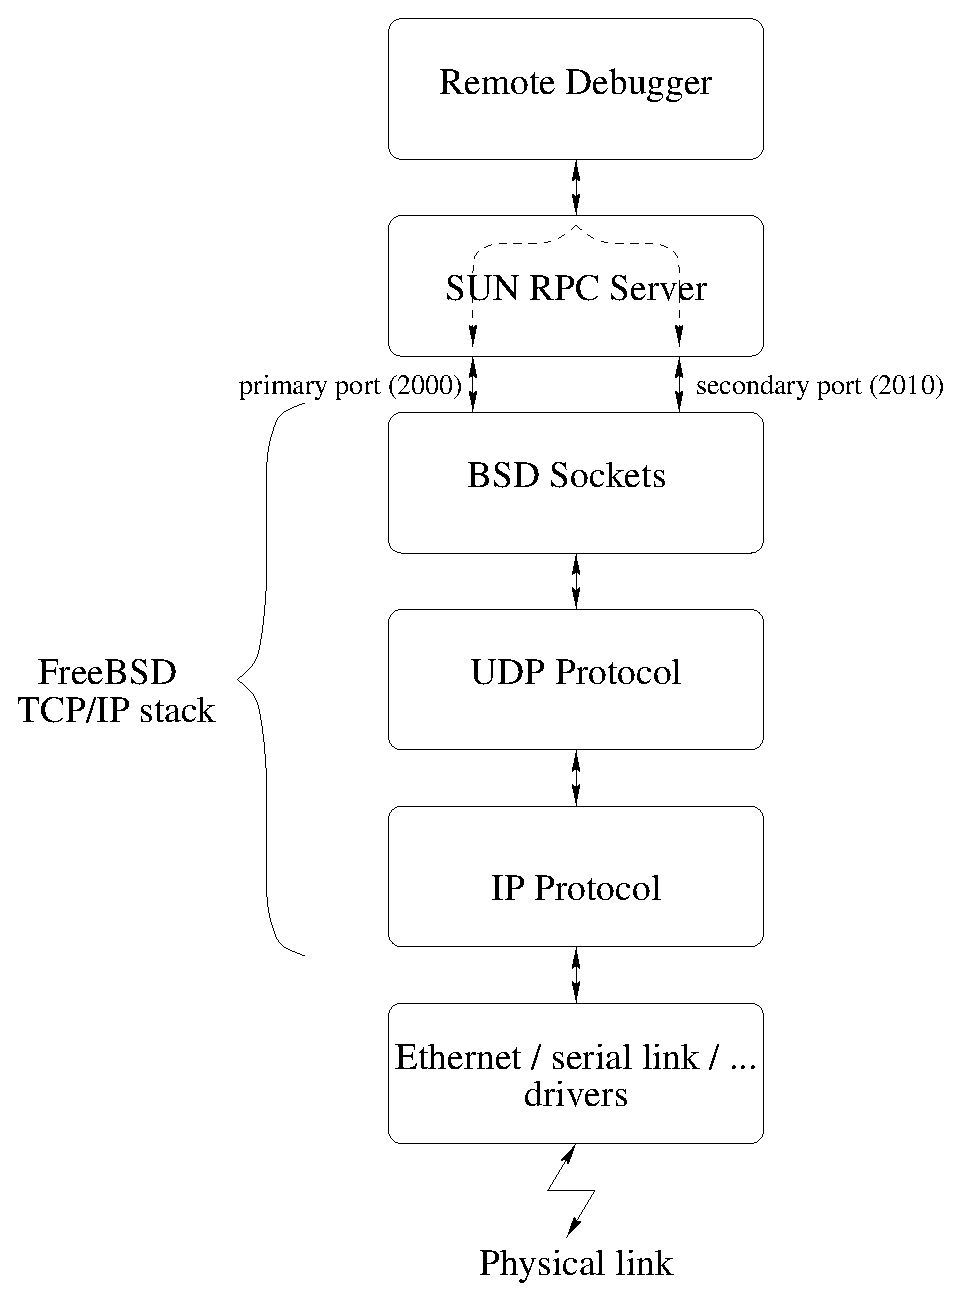
\includegraphics{layers.eps} \par}


\caption{\label{layer}Communication layers}
\end{figure}



\section{\noindent RTEMS Debugger Server Daemon}

\noindent We will describe in this section how this debugger server will be
implemented on RTEMS environment. Our initial target is based on Intel Pentium
and we will use an Ethernet link to communicate between the host and the target.

\noindent The RTEMS remote debugger will be composed by several tasks and exception
handlers :

\begin{itemize}
\item \noindent an initialization task which opens the sockets and runs the SUN RPC
server. This task will also connect the interrupt handlers and launch the communication
task
\item \noindent a communication task which receives the SUN RPC commands, executes
them and sends the result to the GDB client,
\item A debuggee event management task which waits for events. We need a different
task than the command management task in order to be able to still accept commands
while no event has yet occurred for the debuggee. An example could be a continue
command from GDB and then hitting to DEL key to see what is currently going
on on the target side because an expected breakpoint is not caught...
\item \noindent a debug exception handler which manages the hardware breakpoint and
single step exceptions (INT 1 on Intel x86),
\item \noindent a breakpoint exception handler which manages the software breakpoints
exceptions (INT 3 on Intel x86),
\item a default exception handler used to catch every possible errors make on the
target system,
\end{itemize}
\noindent Figure \ref{remote debugger tasks and handlers} represents these
different tasks and handlers. The synchronization between the different task
and exception handlers will be described below in chapter \ref{Synchro_ref}.
Some open issues we have faced for a prototype implementation are described
in chapter \ref{Open_issue_ref}. The temporary workaround we chose are described
in chapter \ref{Workaround_ref}.


\subsection{\noindent The INITIALIZATION task}

\noindent This is the task that must be executed at the boot phase of RTEMS.
It initializes the debug context. It must :

\begin{itemize}
\item \noindent open the UDP sockets,
\item \noindent run the SUN RPC server main loop,
\item \noindent create the COMMAND MANAGEMENT task,
\item \noindent connect the DEBUG EXCEPTION handler,
\item \noindent connect the SOFTWARE BREAKPOINT handler,
\item \noindent delete itself.
\end{itemize}
\noindent If an error occurs at any step of the execution, the connections established
before the error will be closed, before the initialization task deletes itself.


\subsection{\noindent The COMMAND\_MNGT task}

\noindent This task is in charge of receiving the SUN RPC messages and executing
the associated commands. This task must have an important priority because it
must be executed each time a command message comes from the debugger. It must
be executed even if one or both exception handlers are executed. But the COMMAND
MANAGEMENT task must not block the TCP/IP module without which no message can
be received.

\noindent When not executing a command, this task is waiting for a SUN RPC message
on the primary port. This idle state blocks the task, so the other active tasks
can run. Once a message comes from Ethernet via the primary port, the COMMAND
MANAGEMENT task wakes up and receives the message which is a request from GDB.
This request is sent to the SUN RPC server code which extracts the command and
its arguments, executes it and, if needed, sends a result to GDB. After having
performed these actions, the task sleeps, waiting for another message. 

\noindent A particular case is the reception of the ATTACH command : in this
case the COMMAND\_MNGT task creates the EVENT\_MNGT task described below before
going to wait on UDP socket again.


\subsection{The EVENT\_MNGT task}

This task is in charge of managing events happening on the debuggee such as
breakpoint, exceptions. This task does a basic simple loop waiting for event
on a synchronization variable. It is waken up by exception handlers code. It
then signals GDB that an event occurred and then go sleeping again as further
requests will be processed by the COMMAND\_MNGT task.


\subsection{\noindent The DEBUG EXCEPTION handler}

\noindent This handler is connected to the DEBUG exception (INT 1 on Intel ix86).
This exception is entered when :

\begin{itemize}
\item \noindent executing a single-step instruction,
\item \noindent hardware breakpoint condition is true,
\end{itemize}
\noindent These events will be treated by the debugger because they are the
primary event used when debugging a software for instruction stepping. In both
cases, the DEBUG EXCEPTION handler code is executed. Please note that the execution
context of the exception handler is the supervisor stack of the task that generated
the exception . This implies :

\begin{itemize}
\item \noindent We may sleep in this context,
\item We have as many possible execution context for the DEBUG EXCEPTION handler as
we need to,
\item When we enter the high level exception handler code, a normalized exception
context has been pushed on the system stack and a pointer to this context is
available as the first argument (cf c/src/exec/score/cpu/i386/cpu.c for more
details),
\end{itemize}
\noindent First the exception handler wakeup the EVENT\_MNGT task. Then it will
cause the faulting thread to sleep on a synchronization object. As soon as GDB
receives the event notifying that the debuggee status has changed, it will start
sending requests to get the debuggee status (registers set, faulty task id,
...). These requests are handled by the COMMAND MANAGEMENT task. When this task
receive a PTRACE\_CONT command it will resume the execution of the task that
caused the exception by doing a V on the synchronization object. 


\subsection{\noindent The BREAKPOINT EXCEPTION handler}

\noindent This handler is connected to the BREAKPOINT exception (INT3 on Intel
Ix86). Each time the debugger wants to place a software breakpoint in the debuggee,
a debuggee opcode is temporarily replaced by an instruction causing BREAKPOINT
exception (the ``INT 3'' instruction on Intel ix86). When ``INT 3'' is executed,
the BREAKPOINT handler is executed. Otherwise, the exception processing is the
same than the one described in previous section.


\subsection{\label{Synchro_ref}Synchronization Among Tasks and Exception Handlers}

The previous chapters have presented a simplified and static view of the various
tasks and exceptions handlers. This chapter is more focussed on synchronization
requirements about the various pieces of code executed when RGDBSD is operating.


\subsubsection{Implicit Synchronization Using Task Priorities}

This chapter is relevant on Uniprocessor System (UP) only. However, it will
also list the requirements for explicit synchronization on Multi-processor Systems
(MP). Below are the task priorities sorted by high priority. They are not supposed
to be equal :

\begin{enumerate}
\item Network Input Task. This is the highest priority task. This can be regarded
as a software interrupt task for FreeBSD code,
\item RGDBSD command task. As this task waits on UDP sockets, it shall not prevent
the previous task from running. As the main debug entry point, it should preempt
any other task in the system,
\item RGDBSD event task. This task should preempt any task but the two mentionned
before to signal a debug event to GDB. The command task shall be able to preempt
this task for emergency command such as DEL, or REBOOT,
\item Applications tasks (task we are able to debug),
\end{enumerate}
Using theses priorities eliminates the need for adding more synchronization
objects in the next section. My belief is that symmetric MP support will require
more important change in the RTEMS than RGDBSD itself like multiple scheduler
queues, task to processor binding for non symmetric IO, use a different implementation
for \emph{task\_disable\_preemption}, ...


\subsubsection{Explicit Synchronization}

This chapter will describe the synchronization variables that need to be implemented
in order to sequence debug events in a way that is compatible with what GDB
code expects. The root of the problem is that GDB code mainly expects that once
a debug event has occurred on the debuggee, the entire debuggee is frozen and
no other event will occur before the CONTINUE command is issued. This behavior
is hard to achieve in our case as once we hit a breakpoint, only the task that
hits the breakpoint will be asleep on a synchronization object. Other tasks
may hit other breakpoints while we are waiting commands from GDB generating
potential unexpected events. There is a solutions if RGDBSD itself use RTEMS
threads to fix this problem by creating a task that loops forever at a priority
superior to any debugged task but below RGDBSD task priorities. Unfortunately
this will not work for the case we use the nano-kernel implementation and we
think it is better to study synchronization problems now. We also expects that
multi-thread debug support hardening in GDB will remove some event serializations
requirements. Here is the list of synchronization variables we plan to use and
their usage. They are all regular semaphores. They are not binary semaphores
because the task that does V is not the task that has done the P.

\begin{itemize}
\item \emph{WakeUpEventTask} : used by exception handler code to wake up the EVENT\_MNGT
task by doing a V operation on this object. When target code is running normally
the EVENT\_MNGT task sleeps due to a P operation on this semaphore,
\item \emph{SerializeDebugEvent} : used to serialize events in a way compatible to
what GDB expects. Before doing a V operation on \emph{WakeUpEventTask,} the
exception handler does a P on this semaphore to be sure processing of another
exception is not in progress. Upon reception of a CONTINUE command, the COMMAND\_MNGT
task will issue a V operation so that the exception code can wake up EVENT\_MNGT
task using the mechanism described above,
\item \emph{RestartFromException} : (in fact one semaphore per task) used by exception
handling code to put a faulty task to sleep once it has generated an exception
by doing a P operation on this semaphore. In the case the exception was generated
due to a breakpoint, GDB command will modify back the BREAKPOINT opcode to the
original value before doing the CONTINUE command. This command will perform
a V on this semaphore. In the case it is a real non restartable exception (faulty
memory reference via invalid pointer for example), GDB will not allow to restart
the program avoiding any loop. So not special analysis of cause of exception
is foreseen as far as RGDBSD code is concerned,
\end{itemize}

\subsection{\label{Open_issue_ref}Open Issues}

Here are some problems we have faced while implementing our prototype :

\begin{description}
\item [Protected~ReadMem/WriteMem~(I1)]: A GDB user can request to see the content
of a corrupted pointer. The request PEEK\_DATA will be performed by the COMMAND\_MNGT
task. It shall not enter the default exception handler set by RGDBSD or it will
cause a dead lock in the RGDBSD code. Replacing the default exception vector
before calling \textbf{readMem/writeMem} can be temporarily sufficient but :

\begin{itemize}
\item It will never work on MP system as it will rely on task priorities to insure
that other task will not cause exceptions while we have removed the default
exception handler,
\item This feature should not be usable in RGDBSD only but also by an embedded debugger
that may run without any task. It is also unavoidable in case of protected memory
and in this case no priority mechanism can be used,
\item In the case of using RGDBSD code on a dedicated nano kernel, this code will
be called from interrupt level and we need a way to be sure we can debug other
interrupts that may also cause exceptions,
\end{itemize}
\item [ATTACH~Command~Implementation~(I2)]: After the \emph{target rtems symbolic\_ip\_target\_name}
command, the normal operation is to issue an \emph{attach lid} command where
\emph{lid} represents a valid execution context. For Unix this is a process
id, for other multi-tasking system this is the id of a thread. After the attach
command, GDB expects to be waken up in the same manner as it is for normal events.
Once waken up it expects to have a complete register context available and also
that the target task is in a stopped state and that it can restart it using
the regular CONTINUE command. In RTEMS there is a way to get force a thread
to become inactive via \emph{rtems\_task\_suspend} but no way to get the full
registers set for the thread. A partial context can be retrieved from the task
\emph{Registers} data structure. On the other hand, relying on \emph{rtems\_task\_suspend}
will be a problem for the nano-kernel implementation.
\item [Stopping~Target~System~(I3)]: Allthough it might not be obvious, most of the
actions made by a GDB user assume the target is not running. If you modify a
variable via the \emph{set variable = value} command you expect that the value
is the one you have put when restarting. If a still running task modifies the
same value in the mean time, this may be false. On the other hand, stopping
all the tasks on the target system impose to have a very deep knowledge of the
system. Using an interrupt driven RGDBSD, may facilitate the implementation
on the nano-kernel. 
\item [Getting~Tasks~Contexts~(I4)]: As previously mentionned there is no way to get
tasks execution contexts via the RTEMS API. This is needed when debugging for
example via this classical sequence :

\begin{enumerate}
\item \emph{(gdb) target rtems symbolic\_ip\_target\_name}
\item \emph{(gdb) info threads <=} get a thread list on screen
\item \emph{(gdb)} \emph{attach thread\_id} <= thread\_id is one of the thread in
the list
\item \emph{(gdb) b a\_function\_of\_interest }
\item \emph{(gdb) continue}
\item \emph{(gdb)} \emph{backtrace} <= print the call stack on the screen once we
have hit the breakpoint
\item \emph{(gdb) thread target another\_thread\_li <=} change implicit current thread
value for gdb commands
\item \emph{(gdb)} \emph{backtrace <=} should print the backtrace for the chosen thread
\end{enumerate}
In our execution model, we have a valid context only for the threads that hits
the breakpoint as it has been pushed by the exception handler code. The other
thread is still running and during the various RPC requesting memory access,
it even changes as the COMMAND\_MNGT thread is going to sleep. So the backtrace
command will fail. We must find a way to make this work as it is very usefull
when debugging multi-threaded programs,

\item [Backtrace~Stop~convention~(I5)]: The backtrace command on RTEMS task does not
gracefully terminate as GDB does not find some backtrace termination condition
it expects.
\end{description}

\subsection{\label{Workaround_ref}Workarounds for Open Issues in Prototype}

\begin{description}
\item [(I1)]: Not implemented.We would rather like to work on the formalization of
per thread flags and global flags that are much more general than any kludge
we could implement,
\item [(I2)]: We have tried two solutions in our prototype. The first one was to use
the \emph{idle} thread context contained in the \emph{Registers} task control
block field. The drawback of this solution was that we had to implement specific
code for the continue operation immediately following the attach command. We
then decided to create a dedicated task that will only exist during the attach
phase. This task will call the ``ENTER\_RGDB'' exception. This call will execute
the Exception Handler that saves a valid context and that notifies a change
to GDB. After the first CONTINUE command from GDB, this task will continue its
execution and delete itself,
\item [(I3)]: As explained above in the synchronization chapter, we choose to serialize
events in a way that makes GDB think the system is frozen,
\item [(I4)]: As a temporary fix, we have called \emph{rtems\_task\_suspend} and used
the context switch contex for tasks that are unknown to RGDBSD,
\item [(I5)]: Not Implemented yet. If I remember correctly, setting the frame pointer
to 0 at task initialization for CISC processor solves this problem (ebp = 0x0
on Intel or a6 = 0x0 on 680x0). This should be done in rtems\_task\_create function
in the path to really starts the task for the first time. The processor/system
specific stop condition can be found as macros in the GDB source tree.
\end{description}

\subsection{Output of a Debug Session with the Prototype}

\begin{lyxcode}
GNU~gdb~4.17~Copyright~1998~Free~Software~Foundation,~Inc.~GDB~is~free~software,~

covered~by~the~GNU~General~Public~License,~and~you~are~welcome~to~change~it~and/or~

distribute~copies~of~it~under~certain~conditions.~Type~\char`\"{}show~copying\char`\"{}~to~see~the~

conditions.~There~is~absolutely~no~warranty~for~GDB.~Type~\char`\"{}show~warranty\char`\"{}~for~

details.~This~GDB~was~configured~as~\char`\"{}-{}-host=i686-pc-linux-gnu~-{}-target=i386rtems\char`\"{}.

Attaching~remote~machine~across~net...

Connected~to~net-test.~

\ 

Now~the~\char`\"{}run\char`\"{}~command~will~start~a~remote~process.

\ 

Setting~up~the~environment~for~debugging~gdb.~

(gdb)~attach~1~

Attaching~program:~/build-rtems/pc386/tests/debug.exe~pid~1~

0x230715~in~enterRdbg~()~

(gdb)~info~threads~

There~are~8~threads:~

Id.~~~~~~~Name~~~Detached~~~Suspended

\ 

134283273~Rini~~~No~~~~~~~~~No~<=~current~target~thread~

0x230715~in~enterRdbg~()~

134283272~Evnt~~~No~~~~~~~~~No~

\_Thread\_Dispatch~()~at~/rtems/c/src/exec/score/src/thread.c:315~

134283271~SPE2~~~No~~~~~~~~~No~

\_Thread\_Dispatch~()~at~/rtems/c/src/exec/score/src/thread.c:315~

134283270~SPE1~~~No~~~~~~~~~No~

\_Thread\_Handler~~()~at~/rtems/c/src/exec/score/src/thread.c:1107~

134283269~RDBG~~~No~~~~~~~~~No~

0x230715~in~enterRdbg~()~

134283268~SCrx~~~No~~~~~~~~~No~

\_Thread\_Dispatch~()~at~/rtems/c/src/exec/score/src/thread.c:315~

134283267~SCtx~~~No~~~~~~~~~No~

\_Thread\_Dispatch~()~at~/rtems/c/src/exec/score/src/thread.c:315~

134283266~ntwk~~~No~~~~~~~~~No~

\_Thread\_Dispatch~()~at~/rtems/c/src/exec/score/src/thread.c:315~

(gdb)~b~init.c:89~

Breakpoint~1~at~0x200180:~file~/rtems/c/src/tests/samples/debug/init.c,~line~89.~

(gdb)~c~

Continuing.~

Thread~134283273~(Rini)~has~been~deleted.~

{[}Switching~to~Rtems~thread~134283271~(Not~suspended)~(~<=~current~target~thread~){]}

\ 

Breakpoint~1,~example2~(argument=4)~at~/rtems/c/src/tests/samples/debug/init.c:89~

89~~~~~~~~~~tuto~+=~tuti;~

(gdb)~s~

90~~~~~~~~~~if~(print\_enable2)~

(gdb)~c~

Continuing.

\ 

Breakpoint~1,~example2~(argument=4)~at~/rtems/c/src/tests/samples/debug/init.c:89~

89~~~~~~~~~~tuto~+=~tuti;~

(gdb)~b~init.c:66~

Breakpoint~2~at~0x200128:~file~/rtems/c/src/tests/samples/debug/init.c,~line~66.~

(gdb)~c~

Continuing.~

{[}Switching~to~Rtems~thread~134283270~(Not~suspended)~(~<=~current~target~thread~){]}

\ 

Breakpoint~2,~example1~(argument=4)~at~/rtems/c/src/tests/samples/debug/init.c:66~

66~~~~~~~~~~toto~+=~titi;~

(gdb)~c~

Continuing.~

\ 

{[}Switching~to~Rtems~thread~134283271~(Not~suspended)~(~<=~current~target~thread~){]}

\ 

Breakpoint~1,~example2~(argument=4)~at~/rtems/c/src/tests/samples/debug/init.c:89~

89~~~~~~~~~~tuto~+=~tuti;~

(gdb)~bt~

\#0~~example2~(argument=4)~

~~~~at~/rtems/c/src/tests/samples/debug/init.c:89~

\#1~~0xf0009bd0~in~??~()~

(gdb)~thread~target~134283270

\ 

thread~134283270~{[}SPE1{]},~\_Thread\_Dispatch~()~at~/rtems/c/src/exec/score/src/thread.c:315~

315~~~~~~~~~executing~=~\_Thread\_Executing;~

(gdb)~c~

Continuing.

\ 

Breakpoint~2,~example1~(argument=4)~at~/rtems/c/src/tests/samples/debug/init.c:66~

66~~~~~~~~~~toto~+=~titi;~

(gdb)~detach~

Detaching~program:~/build-rtems/pc386/tests/debug.exe~pid~1~

Warning:~the~next~command~will~be~done~localy!~If~you~want~to~restart~another~remote~

program,~reuse~the~target~command~

(gdb)~
\end{lyxcode}

\section{Conclusion}

In this document we have presented how we envisage to add remote debugging facilities
to RTEMS by implementing a remote debugger daemon for GDB. As any debug implemented
in software, it will have limitation but we are confident that most of them
can be removed by adding separate software components dedicated to debug activity.
We must keep in mind that even with this approach, no software will enable the
debug of code with interrupt entirely masked at processor level and that In
Circuit Emulator (ICE) or use of BDM extension on the target board are the ultimate
way to really debug any portion of an RTOS. BDM support in GDB is still weak
but people are working on it and we may get something better in a near future.

\begin{figure}
{\par\centering \resizebox*{!}{0.98\textheight}{\rotatebox{90}{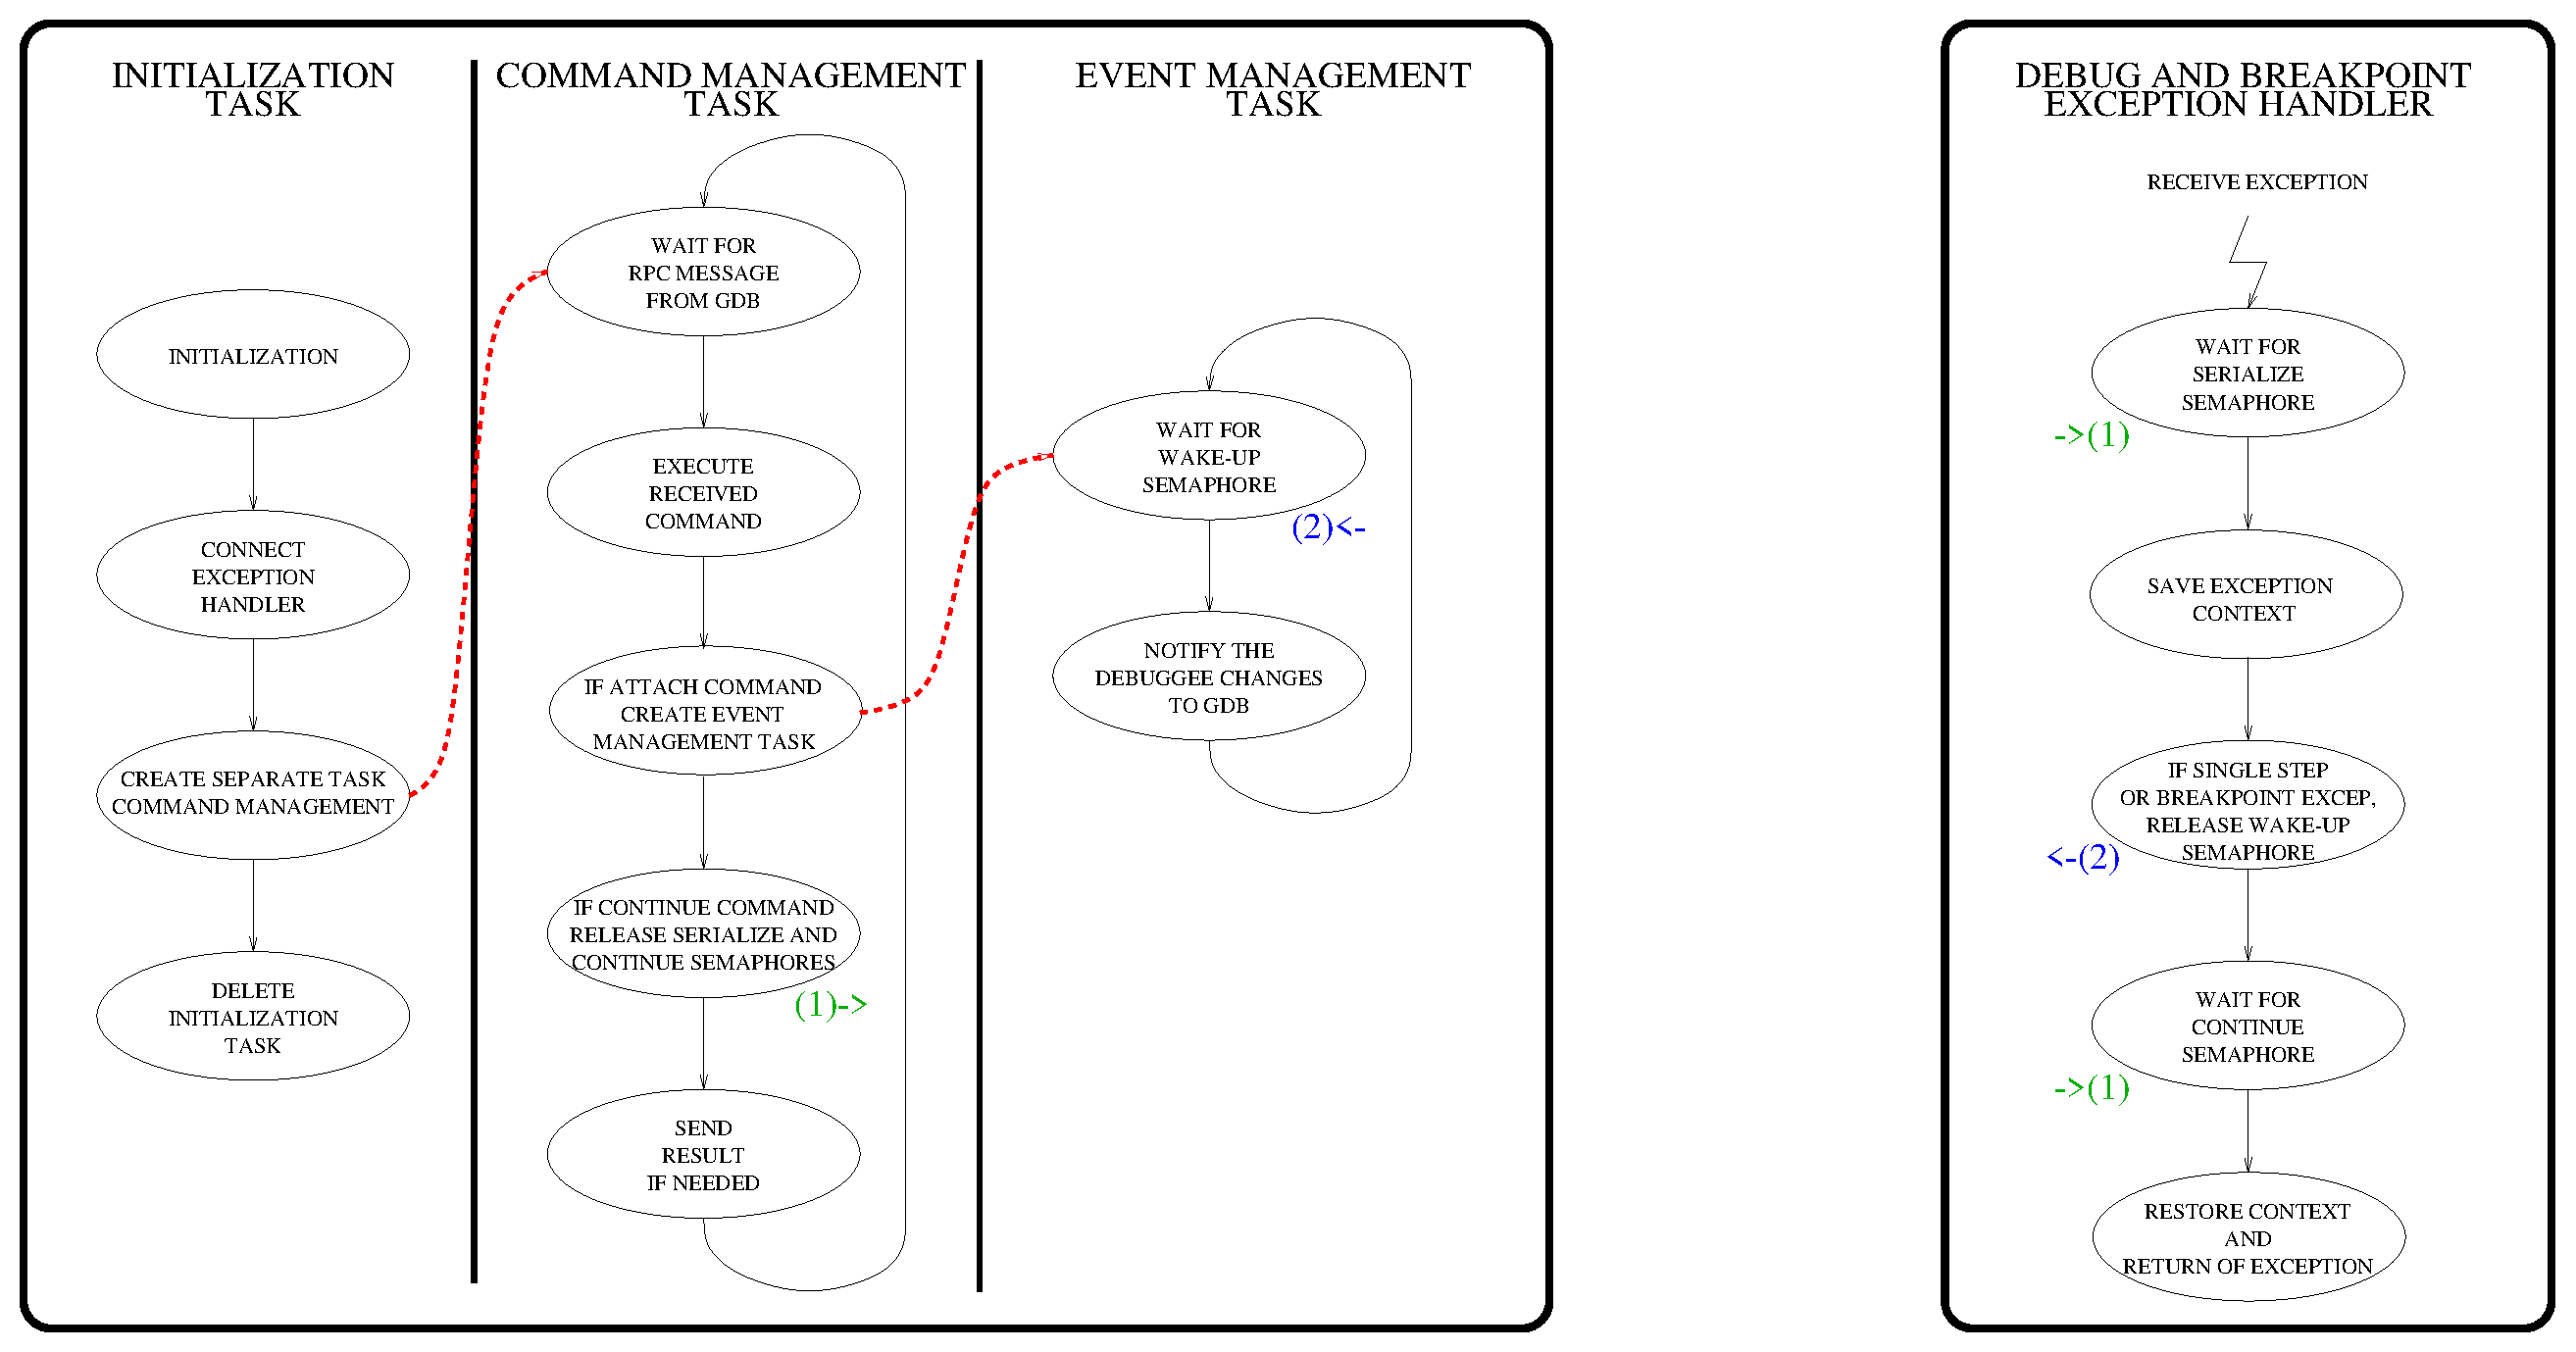
\includegraphics{process.eps}}} \par}


\caption{\label{remote debugger tasks and handlers}remote debugger tasks and handlers}
\end{figure}


\end{document}
